\documentclass[11pt]{article}
\usepackage[utf8]{inputenc}
\usepackage[T1]{fontenc}
\usepackage{fixltx2e}
\usepackage{graphicx}
\usepackage{longtable}
\usepackage{float}
\usepackage{wrapfig}
\usepackage{soul}
\usepackage{textcomp}
\usepackage{marvosym}
\usepackage{wasysym}
\usepackage{latexsym}
\usepackage{amssymb}
\usepackage{hyperref}
\tolerance=1000
\usepackage{color}
\usepackage{listings}
\usepackage{geometry}
\geometry{hmargin=2cm,vmargin=3cm}
\usepackage{fancyhdr}
\pagestyle{fancy}

\lhead{Guía Técnica de ISW}
\rhead{Curso 2011/2012}
\cfoot{Pág. \thepage}

\usepackage{hyperref}

\hypersetup{pdfborder={0 0 0},colorlinks,linkcolor=blue,urlcolor=blue}

\lstset{language=java,frame=single,basicstyle=\footnotesize,breaklines=true,emphstyle=\textbf}
\providecommand{\alert}[1]{\textbf{#1}}

\title{Especialidad de Ingeniería del Software\\ Grado en Ingeniería
Informática\\ Universidad de Cádiz\\ \textbf{Guía Técnica para las Prácticas}}
\author{Daniel Molina Cabrera <daniel.molina@uca.es> \and Juan Manuel Dodero
<juanma.dodero@uca.es>} \date{Curso 2011/2012}


\begin{document}


\maketitle


\setcounter{tocdepth}{2} \tableofcontents \vspace*{1cm} \newpage
\setlength{\parindent}{0pt} \setlength{\parskip}{1ex plus 0.5ex minus 0.2ex}


\section{Descripción del documento} \label{sec-1}



Este documento se plantea como una guía técnica para la realización de las
prácticas y el proyecto de las asignaturas de la especialidad de Ingeniería del
Software en el Grado en Ingeniería Informática y en el segundo ciclo de
Ingeniería Informática. Esta guía es válida para las siguientes asignaturas:

\begin{itemize}
\item Diseño de Sistemas Software (DSS)
\item Ingeniería Web (IW)
\item Implementación e Implantación de Sistemas Software (IISS)
\item \textit{To be completed}
\end{itemize}

La idea de este documento es el de ofrecer una guía que permita a los alumnos/as
de dichas asignaturas reducir los problemas técnicos y centrarse en la
resolución de las prácticas.


\section{Lenguaje Java} \label{sec-2} Las prácticas se realizan en general
empleando el lenguaje de Programación Java. Se ha elegido este lenguaje ya que
es un lenguaje muy extendido, uno de los más usados en el desarrollo de
aplicaciones web de servidor, así como en otros tipos de sistemas ---por
ejemplo, las aplicaciones móbiles para Android se pueden programar usando Java.

Otros puntos a favor es su cercanía al lenguaje (C++) ya aprendido en
asignaturas anteriores, y la existencia de excelentes Integrated Development
Environments (IDE) libres que simplifican mucho el desarrollo.

Tal y como se describe en el apartado de \hyperref[sec-3]{IDEs}, se propone usar
un IDE, para facilitar el trabajo. Además, cada proyecto debe crearse con una
estructura estándar, independiente del IDE. Para ello se empleará la herramienta
\emph{maven}, descrita en el apartado de \hyperref[sec-5]{Maven}.


\subsection{Introducción a Java} \label{sec-2-1}
\label{fd70e36c-20a8-4577-90be-f671166ae3f1}


La sintaxis del lenguaje Java es muy parecida a la de C++. Se recomienda leer el
documento \href{http://www.xtec.es/~acastan/textos/Java.pdf}{Introducción al
Java para programadores C++}.


\subsection{Bibliotecas Java} \label{sec-2-2} Java, a diferencia de C++,
presenta casi desde sus comienzos una completa biblioteca de clases que
implementan muchas funcionalidades. De momento nos centraremosen las siguientes:

\subsubsection{Clases contenedoras} \label{sec-2-2-1} El manejo de clases
contenedoras ofrecido por C++ mediante la STL presenta dos problemas
principales: El confuso uso de los templates, y la poca utilidad de los mensajes
de error. La biblioteca Java contiene en el paquete \textbf{java.util.\*} un
conjunto de clases contenedores estándar más fáciles de utilizar. Por ejemplo,
Java ofrece las siguientes clases muy útiles:

\begin{itemize} \item \textbf{List} (listas), implementadas como
\emph{ArrayList} (\emph{arrays} en C++) o como \emph{LinkedList} (Listas
enlazadas); \item \textbf{Map}, implementado como \emph{HashMap} (\emph{tabla
hash}); \item \textbf{Set} (colecciones sin repetición). \end{itemize}

Aunque se suelen usar bastante las listas (\emph{List}), los \emph{Map}s son en
ciertos casos más apropiados y permiten simplificar bastante el código.

\subsubsection{Fechas} \label{sec-2-2-2} Es ampliamente reconocido el mal manejo
de las fechas por parte de la biblioteca estándar de Java, por tener un API poco
intuitiva y nada cómoda, en el afán de realizar una biblioteca de fechas
reutilizable para todos los calendarios, y no sólo el gregoriano.

El hecho de que una funcionalidad esté en un API estándar no impide que pueda
utilizarse otra biblioteca. En ese caso, se recomienda el uso de la biblioteca
\href{http://joda-time.sourceforge.net/}{Joda-Time}.

En el apartado \hyperref[sec-5]{añadiendo bibliotecas} se introduce cómo
instalar las bibliotecas.

\subsubsection{Validaciones} \label{sec-2-2-3} En cualquier aplicación, es
importante siempre validar los parámetros introducidos por el usuario y,
especialmente, cuando haya que realizar conversiones, como por ejemplo, una
fecha en formato de cadena.

Para ello es muy útil instalar la biblioteca \textbf{commons} de la fundación
Apache. En dicha biblioteca, existe la clase
\href{http://commons.apache.org/lang/api-2.5/org/apache/commons/lang/Validate.html}{Validate}
que permite métodos que facilitan la comprobación de parámetros (devuelve una
excepción si no se cumple). La idea es similar al uso de \emph{assert} en C/C++.


%\subsection{Implementación de la funcionalidad} %\label{sec-2-3} % %Para poder
ofrecer libertad en el diseño, cada grupo debe de elegir la estructura de clases
que crea más conveniente. %Para poder probar el código de forma homogénea, se
ofrecerá unos interfaces. Dentro del código deberá de existir %clases que
implementen dichos interfaces y que delegen las funcionalidades pedidas a las
clases que implementen %dichas funcionalidades. Se ofrecerá asímismo %pruebas
automáticas que comprueben la funcionalidad utilizando dicho interfaz.


\section{IDE} \label{sec-3} \label{ide}

Una gran ventaja es que existen para Java entornos de desarrollo que permiten
trabajar de forma mucho más cómoda. Entre los distintos entornos destacan dos
que son gratuitos y libres, ambos multiplataforma, con versiones para Linux,
Windows y Mac (gracias a la portabilidad de Java). Ambos están fácilmente
disponibles en la web.

\begin{itemize} \item \href{http://eclipse.org/}{Eclipse} es el IDE libre más
popular. Existes muchas versiones de eclipse personalizadas para distintos
propósitos, como por ejemplo \href{http://www.springsource.org}{SpringSource
Tool Suite}, preparada para el desarrollo con el contenedor Spring y el
framework Grails, basado en Java \item \href{http://netbeans.org/}{Netbeans}, es
el IDE oficial de Sun/Oracle, \end{itemize}

%A su vez, en el campus virtual existe una transparencia sobre el entorno de
desarrollo Eclipse, \emph{Introduccion\_{}eclipse.pdf}, introduciéndolo.

\subsection{Netbeans y Eclipse} \label{sec-3-1} Ambos entornos son muy
completos, y la elección de uno u otro depende en gran parte de preferencias
personales. Eclipse posee una estructura más modular (existen módulos para casi
todo), y Netbeans es más compacto. Esto presenta ventajas y desventajas.

Gracias a la herramienta \emph{maven} la estructura de los proyectos creados,
independientemente del entorno utilizado, será la misma. Por tanto, la
compatilidad está garantizada, aunque es recomendable usar un mismo IDE para
todos los miembros de un equipo de proyecto.

Asímismo, la existencia de Mylyn para la gestión de tareas hace Eclipse más
recomendable para usar, pues ayuda no sólo en la gestión de la construcción del
código, sino también en tareas de gestión del proyecto asociadas al proceso de
desarrollo.
 
\subsection{Características comunes} \label{sec-3-2} Las funcionalidades más
usuales de estos entornos son: Editar código fuente con resaltado de sintaxis,
mantener abiertos múltiples ficheros de proyecto, encargarse de construir
(compilar y ejecutar los programas) sin necesidad de crear un \emph{Makefile} o
algo similar \emph{a mano}), pasar las pruebas automáticas que se hayan
definido,\ldots{}.

Otra opción que ambos IDEs admiten es la inclusión de un depurador de código.
Para poder terminar las prácticas correctamente y a tiempo \emph{es muy
importante saber utilizar el depurador}. Es una herramienta básica de todo
desarrollador, sin la cual se tardaría demasiado.

Ambos entornos ofrecen ciertas características avanzadas, que se describen a
continuación.

\subsubsection{Autocompletado} \label{sec-3-2-1}

A menudo es pesado tener que recordar el nombre de las variables y/o métodos.
Esta repetición es proclive a errores. Esto es especialmente molesto en Java, ya
que es un lenguaje bastante verborréico. Una funcionalidad que se vuelve
necesaria es la del autocompletado. En ambos IDEs, al empezar a escribir una
variable y pulsar \textbf{CTRL+SPACE}, se muestran los posibles nombres, a
elegir. Si es únicamente uno, se completa. Con esta característica no hay
excusas para no usar variables con nombre muy descriptivo, aunque sean más
largas de escribir :-).

Otra opción muy interesante del autocompletado es que cuando se desea llamar a
un método de un objeto, basta con pulsar su nombre seguido del punto
(\textsf{objeto.}) y pulsar \textbf{CTRL+SPACE}. Esto muestra los distintos
métodos posibles (métodos públicos de esa clase), incluyendo los parámetros
necesarios. Es muy útil a la hora de saber las posibilidades que brindan las
clases.

\subsubsection{Detección y resaltado dinámico de errores} \label{sec-3-2-2}

Es una característica muy útil que evita muchas compilaciones. Conforme se va
escribiendo, va detectando posibles errores sintácticos, y los marca de color
rojo. Así, una vez terminado un trozo de código, sentencia o función, la
existencia de marcas rojas indica errores a arreglar. De esta manera, se pueden
arreglar errores sin esperar a compilar el proyecto.


\subsubsection{Refactoring} \label{sec-3-2-3}

A menudo es necesario hacer cambios en el código, no para aumentar el rendmiento
o la escalabilidad, sino para mejorar el diseño y hacerlo más flexible. A estos
cambios se les denomina \textit{refactoring} o rediseño. Es una técnica
consistente en una serie de cambios pequeños, para mejorar la flexibilidad, el
mantenimiento y la legibilidad del código.

Dado que introducir un pequeño cambio (como, por ejemplo, cambiar el nombre de
un método o clase) puede ser muy laborioso, los IDEs actuales ofrecen utilidades
para ello (por ejemplo, renombrar una clase o método cambiando automáticamente
todas sus referencias del proyecto.

\subsubsection{Pruebas automáticas} \label{sec-3-2-4}

Para comprobar continuamente el correcto funcionamiento de cualquier
funcionalidad implementada, es necesario que el proyecto pase determinados casos
de prueba automáticos. Estos casos de prueba conviene pasarlos periódicamente,
cada vez que se haga una reconstrucción, o incluso automáticamente desde un
servidor de \emph{integración continua}.

Los IDEs permiten facilitar la creación de los casos de tests, creando el
esqueleto, pudiendo centrarse el programador en dar cuerpo a los métodos de
prueba con las funcionalidades deseadas que se pretenden probar. Tambien
permiten facilitar su ejecución con un simple click u orden a maven, y comprobar
el número de tests pasados (y en qué ejemplos no se han pasado los tests).

\subsubsection{Gestión de bibliotecas} \label{sec-3-2-5}

Como se usará \hyperref[sec-5]{Maven} para instalar las bibliotecas, también se
delegará en ésta la gestión de dependencias con respecto a bibliotecas externas
que necesitemos para la compilación y ejecución de nuestro proyecto. Ambos IDEs
permiten una integración muy sencilla de un proyecto con la estructura
determinada por maven.

Antes de poder trabajar y/o crear un proyecto maven bajo Eclipse, es necesario
instalar el plugin \href{http://m2eclipse.sonatype.org/}{M2Eclipse}. Dicho
plugin, al igual que otros, pueden instalarse directamente desde el propio
entorno de Eclipse.

En primer lugar, es necesario crear el nuevo proyecto como un proyecto Maven,
para poder usarlo. Si se crea el proyecto como otro tipo de proyecto no podrá
usarse, habrá que crear el proyecto de nuevo.

Un vez creado el proyecto, se puede incluir dependencias de las bibliotecas que
queremos, indicando incluso el número de versión mínimo requeridad. Ambos IDEs
permiten buscar las bibliotecas opotunas.

Por defecto, ambos entornos poseen una serie de repositorios predefinidos de
bibliotecas, pero puede aumentarse esa lista para poder instalar bibliotecas
adicionales. Todas las bibliotecas recomendadas en esta guía poseen un
repositorio maven. El concepto es muy similar a añadir un nuevo repositorio
Ubuntu usando \emph{apt-add-repository}. Para acceder al repositorio sólo hay que seguir los
enlaces de las bibliotecas de la documentación.


En los enlaces siguientes se puede ver cómo se puede \href{http://m2eclipse.sonatype.org/adding-project-dependencies-in-m2eclipse.html}{añadir bibliotecas en Eclipse} y \href{http://wiki.netbeans.org/MavenBestPractices}{añadir bibliotecas en Netbeans} usando Maven.


\subsubsection{Herramientas de trabajo en grupo}
\label{sec-3-2-6}

Los entornos permiten facilidades de trabajo en grupo, como el soporte de los
sistemas de control de versiones como \emph{Subversion} o \emph{Git}.


\section{JUnit: Pruebas automáticas} \label{sec-4}

Inicialmente se suelen hacer pruebas
\emph{a mano} del código programado (es decir, invirtiendo horas haciendo pruebas con valores
introducidos a mano y comprobados los resultados). Esa forma de hacer pruebas es
intuitiva, pero es demasiado laboriosa y, sobre todo, difícilmente reproducibles. 

Otra forma de abordar las pruebas es mediante el empleo de programas automáticos
que realicen pruebas. Esto permite probar de forma periódica la funcionalidad
implementada, y tener ejemplos directos cuando no funciona de forma correcta (es
más fácil de depurar al tener ona región pequeña de código que no funciona
correctamente).

En Java, esta funcionalidad se suele implementar por medio de la biblioteca
\href{http://junit.sourceforge.net/}{JUnit}, aunque hay otras alternativas. Pueden verse algunos
\href{http://www.slideshare.net/tom.zimmermann/unit-testing-with-junit}{ejemplos} del uso de jUnit. La idea es crear clases adicionales con distintos métodos encargados de
probar el código. \textbf{JUnit} se diseñó para crear pruebas de unidad, por lo
que es común tener, por cada clase que ofrece una funcionalidad determinada, una clase
Test que asegura que el resultado sea el esperado, para distintas
situaciones o datos de entrada a dicha funcionalidad.


\section{Maven: Añadiendo bibliotecas} \label{sec-5} \label{maven}

Un primer problema a la hora de trabajar con un IDE y con un \emph{framework}
(como los \emph{frameworks webs} para Java) es que cada uno de ellos implica una
determinada estructura de ficheros y directorios, haciendo difícil compilar y/o
desarrollar sin tener dicho entorno. Otro problema que se presenta es el de la instalación de bibliotecas, problema muy dependiente de cada una de ellas.

Ambos motivos suelen obligar, para compilar el proyecto, a tener que usar el mismo IDE con el que éste se desarrolló. Para resolverlo surgió un estándar de compilación,
denominado \textsf{ant} (equivalente al uso de \textsf{make} para C/C++). Dicho
programa, parte de una definición en un fichero \emph{xml} denominado
\textbf{build.xml} (similar a un \textit{makefile}) que permite definir las dependencias.

Con el uso de \textbf{ant}, mejoró el proceso, pero no se resolvió el problema
de una estructura común ni facilitar la instalación de bibliotecas.\href{http://maven.apache.org/}{Maven} surgió como una solución a este problema. Maven es un sistema que ofrece las mismas funcionalidades que \textbf{ant} (de hecho, lo utiliza internamente) pero presenta ventajas adicionales.

Explicar el uso de \textbf{Maven} excede las pretensiones de esta guía, por lo
que paso simplemente a comentar dos aspectos importantes para su puesta en práctica.


\subsection{Definición de la estructura} \label{sec-5-1}

Al crear el proyecto como un proyecto Maven, el propio sistema se encarga de
crear una estructura de ficheros y directorios que es estándar. Por tanto, una
vez creado, es posible compilarlo sin necesidad de tener el IDE instalado,
únicamente con Maven. A su vez, Maven también permite definir
fácilmente estructuras necesarias para desarrollar en determinados
\emph{frameworks} específicos, facilitando mucho su desarrollo (puede generar el esqueleto
de la casi totalidad de \emph{frameworks web}).

\href{http://www.youtube.com/watch?v=5Tp3XCEfMGk}{Ejemplo en video usando
m2eclipse}.


\subsection{Instalar bibliotecas} \label{sec-5-2}

Cualquier usuario de Linux agradecerá la facilidad de instalar aplicaciones
directamente por medio de un conjunto de repositorios. Esto permite no sólo un
lugar en donde encontrar la aplicación, sino que también permite, a la hora de
desarrollar una aplicación que dependa de una biblioteca, poder indicar explícitamente dicha
dependencia. De esta forma, cuando se solicita la instalación de la aplicación,
automáticamente se descargan e instala también las bibliotecas de las que
depende, haciendo el proceso de instalación y despliegue muy sencillo tanto para usuarios
como para desarrolladores.

Maven permite realizar esta misma tarea. Por medio del sistema Maven (se puede
hacer desde el propio IDE) se puede indicar que una aplicación requiere una
determinada biblioteca. Así, a la hora de compilar y/o ejecutar el programa,
maven instalará las bibliotecas, si no están ya instaladas, por medio de
repositorios externos.

Esto permite que a la hora de distribuir un proyecto \emph{maven} sólo sea
necesario distribuir vuestro código, sin preocuparse de las bibliotecas. Además, permite indicar la versión de las bibliotecas, evitando cualquier tipo de problema de versiones. Esto, aunque algo más complejo desde un punto de vista técnico, con el uso de IDEs que soportan este sistema acaba
siendo más sencillo que instalar las bibliotecas a mano. Se puede ver su uso, muy similar, tanto en
\href{http://m2eclipse.sonatype.org/adding-project-dependencies-in-m2eclipse.html}{Eclipse}
como en \href{http://wiki.netbeans.org/MavenBestPractices}{Netbeans}. 

Para crear un proyecto maven e instalar dependencias, puede verse el siguiente video de
\href{http://www.youtube.com/watch?v=IRKu8_l5YiQ}{adición de dependencias en m2eclipse}.

\section{Persistencia} \label{sec-6}
\label{librerias}

No serviría de nada una aplicación que no almacenase sus datos para que
estuviesen disponibles en las siguientes ejecuciones. Un enfoque directo sería el uso de una Base de Datos (BD) y guardar los datos
en ella. Afortunadamente, en el API de Java se ofrece un interfaz común llamada JDBC para
las distintas bases de datos, por lo que toda biblioteca que funcione bajo Java
es independiente de la base de datos que tengamos instalada, pudiendo cambiar
una por otra simplemente cambiando la configuración. Es decir, no existen
dependencias innecesarias entre la base de datos concreta y el código de la
aplicación.


Existen varios tipos de bases de datos, apropiadas para distintos tipos de aplicaciones. 

\begin{itemize}

\item Por un lado, las aplicaciones simples pueden usar bases de
datos empotradas, en las que es la propia biblioteca de Java la encargada de
gestionar los datos, sin necesidad de instalar un proceso aparte de SGBD.

\item Por el otro, las aplicaciones más complejas (como las aplicaciones web) suelen requerir un sistema
de BD externo, que permita compartir información entre distintas aplicaciones.

\end{itemize}

En el caso de las BD relacionales, se puede acceder directamente a la Base de Datos
haciendo uso del SQL, o por medio de un framework ORM (\emph{Object Relational Mapping}), que permita asociar
cad objeto de una clase con las tablas de la Base de Datos donde se guarda el estado persistente de estos objetos (esto es, los valores de sus atributos que deban sobrevivir entre sesiones), y permita recuperar y almacenar los objetos en la base de datos. Un ejemplo de motor de ORM muy popular bajo Java es el
\href{http://hibernate.org}{Hibernate}. En Java es muy común el uso del interfaz JPA (Java Persistence API) para inteoperar entre la aplicación y el motor ORM, dado que entre ambos se establecen dependencias que hay que resolver ordenadamente definiendo interfaces estables.

\subsection{Conceptos generales}
\label{sec-6-1}


Aunque existen muchos tutoriales libremente disponibles, no está de más
introducir algunos conceptos asociados para el hibernate.
%\begin{center} 
\includegraphics[width=.6\textwidth]{hibernate.png} \end{center}
En origen, la idea de hibernate es permitir almacenar y recuperar un
objeto Java en una base de datos relacional. Aunque permite guardarlas en distintos
tipos de bases de datos, nos centraremos en MySQL para trabajar.
Sine mabrgo, para depurar podemos usar por ejemplo una base de datos empotrada, no relacional, ya que suele ser más rápido.

\begin{center}
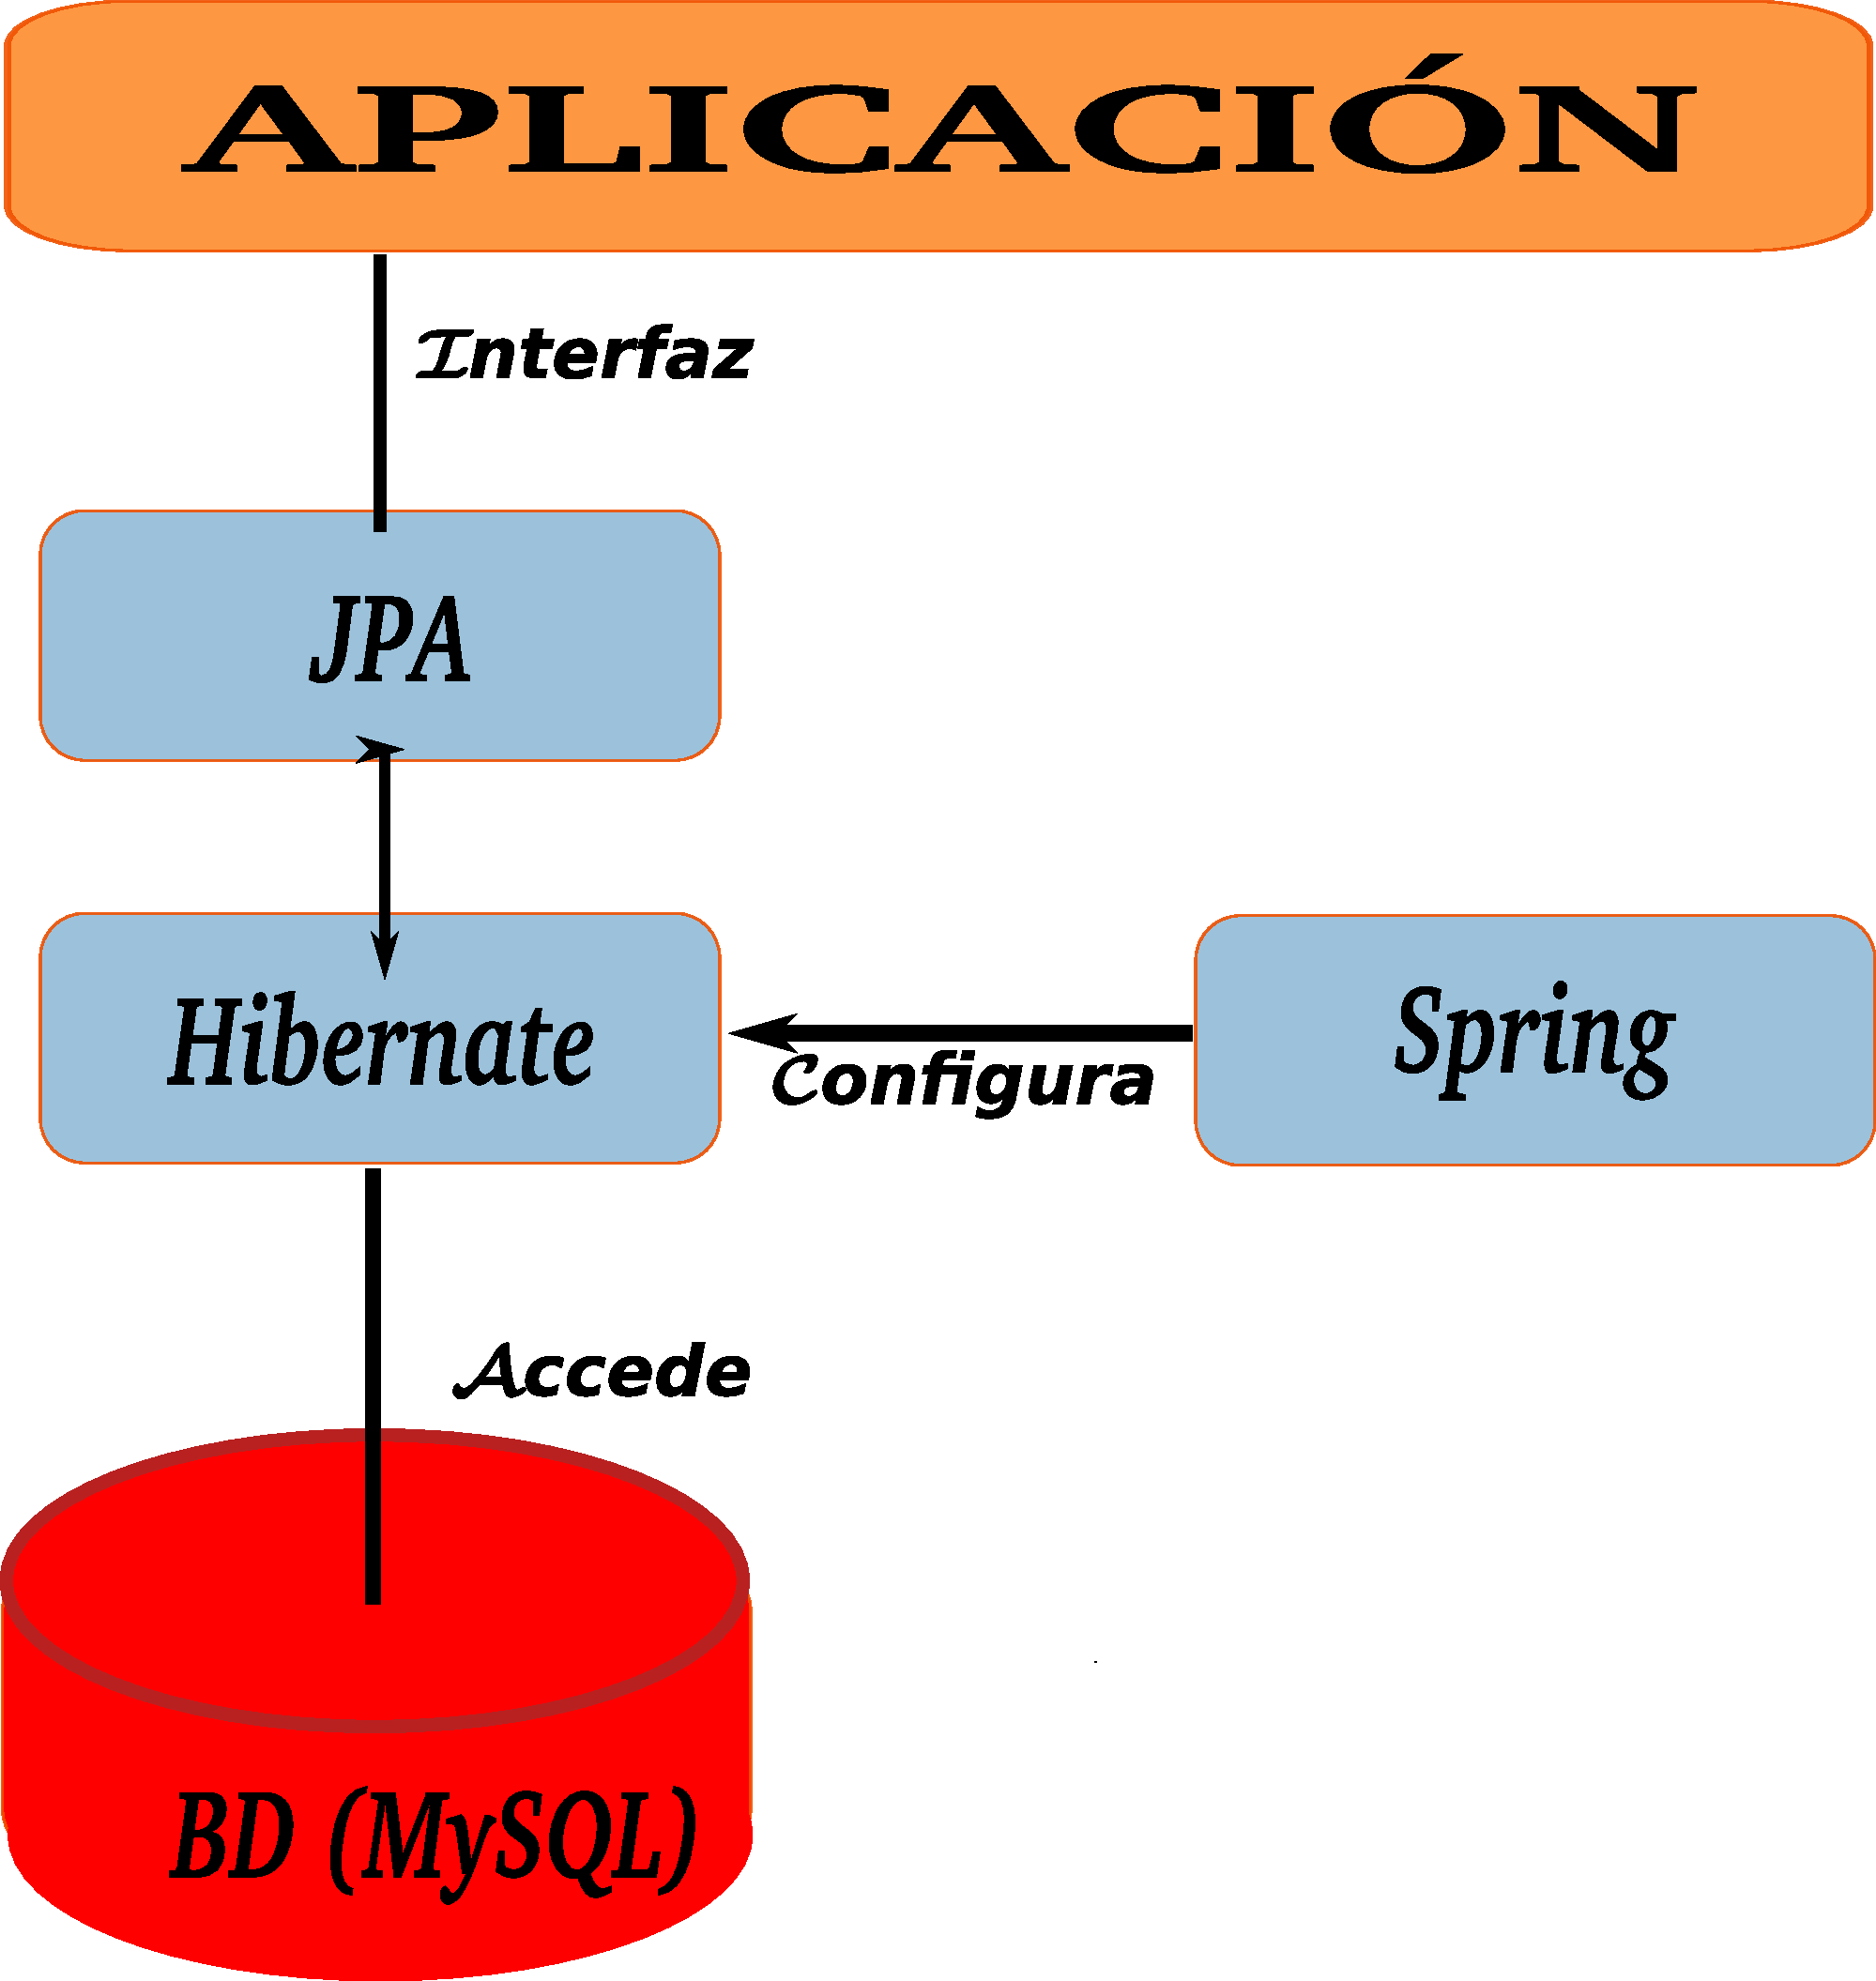
\includegraphics[width=.6\textwidth]{esquemahibernate.pdf}
\end{center}

\begin{itemize}

\item La aplicación o biblioteca debe concoer y utilizar una interfaz estándar JPA que es implementada por Hibernate, que es la que se conectará finalmente con la Base de Datos.

\item La aplicación será configurada por otro componente de biblioteca, denominado Spring, ya ofrece un método de configuración más flexible y cómodo basado en la inyección de dependencias.

\end{itemize}


\subsection{Definición de clases ORM} \label{sec-6-2}

Para poder guardar un objeto de una clase en una base de datos, es necesario establecer la
correspondencia entre los atributos de dicha clase y las columnas de las tablas
en donde se almacenan. Existen dos formas de proceder. Por un lado, el formato
clásico es definir el objeto sin ningún tipo de información y, en un fichero xml
aparte (persistence.xml), almacenar dicha relación. Sin embargo, la tendencia
actual (y nuevo estándar) es incrustar en el código fuente en Java una serie de \emph{tags} (que empiezan por @) que permite señalar dicha correspondencia.

La clase no tiene por qué heredar de ninguna otra clase en particular, y deben tener bien definidos los
atributos a guardar, con sus métodos de acceso get/set correspondientes. Para que el sistema almacene la clase hay que añadir los siguientes atributos:


\begin{description}

\item[@Entity] Define que los objetos de la clase correspondiente se almacenará en la BD. 

\item[@Table(name=''\emph{tablename}'')] Define el nombre de la tabla asociada a dicha entidad (si no se indica, éste coincidirá con el nombre de la clase).

\end{description}


Luego, antes de la declaración de cada atributo se pueden indicar tags que definen su semántica en cuanto al almacenamiento en BD:

\begin{description}

\item[@Id @GeneratedValue] Permite definir el atributo anexo como clave primaria de la tabla. Se autogenerará su valor con cada nuevo objeto.

\item[@Column(name=''\emph{name}'', nullable=true/false)] Permite señalar el nombre de la columna que guardará  el valor, permitiendo indicar si se admite valor nulo o no en la Base de Datos. 

\item[@Basic(optional=true/false)] Permite indicar al ORM si el atributo puede ser nulo o no.


\end{description}

Un par de ejemplos:

\begin{lstlisting}
@Entity @Table(name="author")
public class Author {

  @Id
  @GeneratedValue long id;
  @Column(name="name", nullable=false)
  @Basic(optional=false)
  private String name;

  @Column(name="country", nullable=false)
  @Basic(optional=false)
  private String country;
  ...

}
\end{lstlisting}


¿Cómo se pueden reflejar las asociaciones entre objetos, es decir, las relaciones entre tablas? Se hace por medio de referencias cruzadas. Para indicar que un atributo debe de obtenerse a partir de
otra tabla es necesario añadir otro tipo de información. Los atributos son los siguientes:


\begin{description}

\item[OneToMany(cascade=ALL)] Permite definir que el atributo siguiente (contenedora) es una referencia. El parámetro \emph{cascade} permite hacer borrados/modificaciones en cascada.

\item[ManyToOne(cascade=ALL, mappedBy=''otherclass'')] Permite indicar que el atributo indicado (anónimo)
referencia a otra clase. La opción mappedBy permite indicar el atributo de la otra clase (si la relación es biyectiva).

\end{description}


Se puede consultar más información en el
\href{https://en.wikibooks.org/wiki/Java_Persistence/Relationships}{Wikibook
sobre relaciones usando JPA}. Un ejemplo sencillo sería indicar que un libro
puede tener un (único) autor se reflejaría de la siguiente forma.

\begin{lstlisting}
@Entity
@Table(name="book")
public class Book {
  ...
  @ManyToOne(optional=false, cascade=CascadeType.ALL)
  private Author author;
  ...
}
\end{lstlisting}


\subsection{Uso de la Base de Datos} \label{sec-6-3}

Para acceder a la BD, una vez definidas las clases que vamos a
relacionar en la BD, necesitamos un objeto \textsf{session} de tipo
\textsf{SessionFactory} (en la sección de \hyperref[sec-6-4]{configuración} vemos cómo obtenerlo).


\subsubsection{Recuperar un objeto} \label{sec-6-3-1}

Si tenemos el \emph{id} de un objeto, podemos recuperarlo simplemente con
\emph{session.load(Class, id)}. Por ejemplo:

\begin{lstlisting}
  session.load(Author.class, id).
\end{lstlisting}

En el caso más frecuente no dispondremos del \textsf{id}, pero sí de un conjunto de
restricciones. Podemos obtenerlas mediante la instrucción \textbf{createQuery}, 
que posee la siguiente sintaxis:

\begin{lstlisting}
  session.createQuery(from XXX as XX where XXX.yy ...)
\end{lstlisting}

Esto permite definir una consulta. A la hora de poner la condición, no se debe 
crear una cadena con los valores concretos, ya que pueden generarse muchos
problemas. La opción es uso de parámetros (que empiezan por el símbolo `:'). Es decir, en vez de hacer

\begin{lstlisting}
  Query q = sess.createQuery("from DomesticCat cat where cat.name = " + name);
\end{lstlisting}


Se debe de hacer de la siguiente forma:

\begin{lstlisting}
  Query q = sess.createQuery("from DomesticCat cat where cat.name = :name");
  q.setString("name", name);
\end{lstlisting}


Los métodos para asignarles valores a los parámetros son: \textsf{setString},
\textsf{setDate}, \ldots{} Se puede consultar la documentación.

Una vez asignado valores a los parámetros, es necesario indicar que se devuelvan
los resultados. Se puede indicar que se devuelva un único resultado, con
uniqueResult (si existe sólo un elemento, devuelve null si no lo encuentra).

\begin{lstlisting}
  ...
  q.setString("name", name);
  Cat cat = q.uniqueResult();
\end{lstlisting}


Otra opción es indicar que se desea un grupo de objetos, mediante el método
\textsf{list}:

\begin{lstlisting}
  ...
  q.setString("race", race);
  List<Cat> cats = q.list();
\end{lstlisting}


\subsubsection{Modificar y guardar un objeto} \label{sec-6-3-2}

Un objeto se modifica recuperando el objeto de la BD, modificando los atributos
que queramos, y volviéndolo a almacenar en la BD.

Un ejemplo sencillo, que cambia para todos los gatos de raza `angola' por `Angola', sería:

\begin{lstlisting}
  List<Cat> cats = session.createQuery("from DomesticCat cat where race = :race").
    setString("race", "angola").
      list();
  for (Cat cat : cats)
    cat.setRace("Angola");
  session.save(cat);
\end{lstlisting}

Para borrar el objeto, existe el método \textsf{delete()}.


\subsection{Configuración} \label{sec-6-4} \label{cfgorm}

Como en todo proyecto Maven, la descarga e instalación de las bibliotecas Hibernate
y Spring se realiza de forma automática por medio del fichero \emph{pom.xml}.

La configuración de la configuración de la Base de Datos se hace por medio del
fichero \textbf{beans.xml} en el directorio \emph{resources}.

\lstset{emph={property,bean,value,class,id,name}}

\begin{lstlisting}
<bean id="myDataSource"
      class="org.apache.commons.dbcp.BasicDataSource"
      destroy-method="close">
  <property name="driverClassName"
            value="com.mysql.jdbc.Driver"/>
  <property name="url"
            value="jdbc:mysql://localhost/databasename"/>
  <property name="username"
            value="usuario"/>
  <property name="password"
            value="clave"/>
</bean>
\end{lstlisting}

Para adaptarlo a otra configuración sólo hay que cambiar las siguientes
propiedades:

\begin{description}

\item[driverClassName] Contiene el nombre de la clase que
conecta con la Base de Datos. No hay que cambiarla si se usa MySQL. Si se
desea usar otra Base de Datos, consultar la documentación de dicha BD.

\item[url] La url contiene la información de conexión. Puede depender de la base
de datos. En este caso sólo se cambiaría el nombre de la base de datos (\emph{database}).
\emph{Localhost} es el servidor local que contiene la Base de Datos,

\item[username] es el usuario con el que se va a acceder a la base de datos (un usuario \emph{normal}, no \emph{root}, pero con todos los permisos para la base de datos indicada).

\item[password] Contraseña del usuario de la base de datos.

\end{description}

Adicionalmente, hay que indicar las clases que se relacionarán con la Base de
Datos (y que deberán de poseer los decoradores @Entity, etc.) Esto se
realiza añadiendo el nombre completo de las clases en la lista de la propiedad
\textbf{annotatedClasses} del fichero \emph{beans.xml}. Un posible ejemplo sería
el siguiente:

\lstset{emph={property,name,list,value}}

\begin{lstlisting}
<property name="annotatedClasses">
  <list>
    <value>org.uca.dss.example.data.Author</value>
    <value>org.uca.dss.example.data.Book</value>
    ...
  </list>
</property>
\end{lstlisting}

Por último, necesitamos que las clases que nos permiten operar con la Base de
Datos contengan un objeto de tipo \textsf{SessionFactory} para poder comunicarse
con la Base de Datos (usando el interfaz JPA). ¿Cómo se puede iniciar ese
objeto (es decir, inyectar dicha dependencia)? Spring es capaz de crear objetos con dicho atributo inicializado. Para ello, es necesario indicarlo en el fichero \emph{beans.xml} con una notación
como la siguiente:

\lstset{emph={bean,id,property,name,ref,class}}

\begin{lstlisting}
<bean id="autores"
      class="org.uca.dss.example.dao.RealAuthors">
  <property name="sessionFactory"
            ref="mySessionFactory"/>
</bean>
<bean id="libros"
      class="org.uca.dss.example.dao.RealBooks">
  <property name="sessionFactory"
            ref="mySessionFactory"/>
</bean> \end{lstlisting}

De esta manera, el atributo \textsf{sessionFactory} estará adecuadamente
iniciado para los objetos creados autores y libros de las clases
correspondientes. Para acceder a dichos objetos dentro del código sólo es
necesario hacer:

\lstset{language=java}

\begin{lstlisting}
ClassPathXmlApplicationContext ctx =
    new ClassPathXmlApplicationContext("beans.xml");
Authors autores = (Authors) ctx.getBean("autores");
Books libros = (Books) ctx.getBean("libros");
\end{lstlisting}

en donde \textsf{Authors} y \textsf{Books} son interfaces (que las clases \textsf{RealAuthors} y \textsf{RealBooks} implementan).


\section{Trabajando en equipo, usando una forja} \label{sec-7}

Para poder trabajar en equipo es necesario el uso de una serie de herramientas
que permita trabajar sobre el mismo proyecto, y evitar tener posibles
conflictos.

Lo primero que hay que hacer es asegurarse que se trabaja sobre el mismo código,
para lo cual es necesario un \hyperref[sec-7-2]{Sistema de Control de
versiones}. Otras opciones que nos permiten las forjas es mantener un \textbf{wiki} en el
que documentar y un \hyperref[sec-7-4]{sistema de tickets}. Este tipo de
herramientas son especialmente importantes ya que permiten trabajar de forma
físicamente separada.


\subsection{Configurando un proyecto} \label{sec-7-1}

Para permitir trabajar físicamente por separado es necesario que toda la información
del proyecto esté disponible en un servidor conectado a internet al que 
accedan sus miembros. Afortunadamente, existen distintos servidores, repositorios y forjas,
libremente disponibles. Un ejemplo sería la forja universitaria de RedIris \href{http://forja.rediris.es}{de red iris}. También existen distintas forjas para otros sistemas de control de versiones, como
\href{http://github.com}{Github}, \href{http://www.assembla/}{Assembla} o \href{http://bitbucket.org}{BitBucket}.

En nuestro caso, dado que vamos a usar el Subversion, y queremos usar un sistema
de tickets, vamos a usar la página web \href{http://www.assembla.com}{Assembla}
que nos permite usar ambos, con un interfaz relativamente sencilla.

El proceso es el siguiente:

\begin{enumerate}

\item Acceder a la web de assembla: \href{http://www.assembla.com}{www.assembla.com}

\item Crear un espacio: Cree un Espacio $rightarrow$ Cree un Proyecto Público $rightarrow$ Hosting de Subversion con Tickets Integrados.

\item Inscribirse como usuario de Assembla.

\begin{enumerate}
  \item Darse de alta como usuario.
  \item Elegir un id para el equipo y el nombre corto del proyecto.
\end{enumerate}

\item Acceder a la url del proyecto.

\end{enumerate}


\subsection{Compartiendo código: Sistema de Control de versiones}
\label{sec-7-2} \label{scv}

No es lo mismo desarrollar código por separado que hacerlo en equipo. Además de las múltiples dificultades
comunicativas y organizativas, se añade la dificultad de operar simultáneamente sobre el mismo
código. Si no se opera sobre el mismo código, es difícil trabajar, ya que hay que
estar enviando los ficheros cambiados, con el riesgo de olvidar enviar ciertos cambios, o hacer cambios incompatibles entre sí, con lo que se puede generar situaciones conflictivas muy difíciles de resolver manualmente.

Desde hace muchos años existe una solución: utilizar un servidor
que guarde vuestro código, y (de manera simplificada) sincronizar vuestro código con dicho servidor.
Existen sistemas que permiten esto, denominados \emph{sistemas de control de
versiones}.

De esta manera, se puede subir siempre todos los cambios realizados, y tener la
confianza de trabajar con el mismo código.

El uso de un Sistema de Control de Versiones permite: 


\begin{itemize}

\item Mantener centralizado el código, evitando el riesgo de que
cada desarrollador tenga una versión diferente. 

\item Que los desarrolladores
puedan acceder siempre al código actualizado. 

\item Mantener todas las
versiones, y no sólo la última versión. De esta manera se permite \emph{volver
atrás} si hay un error. 

\item Los desarrolladores pueden bajarse el código
actual, aplicar cambios, y subir sus cambios al repositorio. 

\end{itemize}


La idea de trabajo es la siguiente:


\begin{itemize} 

\item Primero, se descarga el código del servidor. 

\item Se
hacen cambios locales, hasta tener una versión más avanzada, que al menos
compile. 

\item Se sube el código cambiado al servidor. 

\end{itemize}


Además, en todo momento, se puede descargar la nueva versión del servidor,
detectando posibles cambios incompatibles (colisiones), en cuyo caso avisa de
los cambios incompatibles.

Como se trabaja con los cambios, varios desarrolladores pueden, por ejemplo,
añadir distintos métodos a la misma clase, sin que se produzca ningún problema,
lo cual simplifica mucho el trabajo de integración. Un cambio incompatible sería
que dos desarrolladores cambiasen simultáneamente la misma sentencia, o bloque.

En caso de detectar cambios incompatibles, el seguno desarrollador recibiría un
aviso al intentar \emph{subir} su código, y deberá de adaptar su cambio al
cambio anterior.

Hay que recordar que un sistema de versiones espera un cierto grado de
organización entre los desarrolladores, no es una herramienta de sincronización,
simplemente garantiza coherencia en el código.

Otra opción que permite un sistema de control de versiones, es que guarda todas
las versiones, y no sólo la última versión, con lo que siempre se puede volver a
una versión anterior en el caso de cometer un error en el desarrollo, quitando
el \emph{miedo al cambio}. Además, esto implica que no hay que desactivar código
poniéndolo entre comentarios. Si un código no se utiliza, se debe borrar, ya
que siempre se podria recuperar si es necesario (aunque no suele ser necesario).


\subsubsection{Acceder al repositorio del proyecto} \label{sec-7-2-1}

Dentro de la web del proyecto se indica una URL que permite indicar al
subversion dónde se encuentra el repositorio remoto. Un ejemplo sería la URL
\url{http://subversion.assembla.com/svn/mi-proyecto/}

Dentro de esa URL existe un fichero README y un directorio \emph{trunk}. El
código fuente de nuestra aplicación debe estar en dicho directorio. En nuestro
caso, no se guardará únicamente el código fuente, sino también los ficheros de
configuración (\emph{pom.xml}, \emph{beans.xml}, etc.\ldots{}) necesarios para la construcción y el despliegue de la aplicación. El propio entorno
IDE es capaz de trabajar usando el SCV, por lo que se encargará de añadir dichos
ficheros al repositorio.

\subsubsection{Soporte del IDE de los SCV}
\label{sec-7-2-2}

Existen múltiples sistemas de control de versiones, pero los más utilizados son
\href{http://www.subversion.org}{Subversion} (modelo centralizado) y 
\textbf{Git} (modelo de desarrollo distribuido). En este documento nos centramos en \textbf{Subversion}.

Ambos están soportados por los IDEs recomendados. En Eclipse, se recomienda instalar
el plugin \emph{Subeclipse} para poder gestionar el SVN. Se instala directamente desde la
configuración del eclipse, al igual que cualquier otro plugin.

Para entender su uso, mejor que mirar directamente un tutorial de Subversion
(que explicará cómo usarlo desde la linea de comandos), es mejor aprender cómo se
puede usar en los IDEs (obteniendo una visión más directa). En los enlaces
siguientes hay un \href{http://www.ibm.com/developerworks/opensource/library/os-ecl-subversion/}{tutorial
de Subversion bajo Eclipse} y otro \href{http://netbeans.org/kb/docs/ide/subversion.html}{tutorial de Subversion
bajo Netbeans}.

\subsection{Documentando con Wiki} \label{sec-7-3}

Dado que la documentación de una aplicación (incluyendo la documentación de
diseño) es algo vivo, ¿qué mejor forma que usar la wiki del proyecto para
documentarlo?

En el wiki se debe depositar toda la documentación textual (entregables) relacionada con el proceso de desarrollo de la aplicación, incluyendo los diagramas y permitiendo de ese modo
tener un histórico de la documentación.

\subsection{Sistema de Tickets}
\label{sec-7-4} \label{tickets}

TO-DO\ldots


\end{document}